\documentclass[11pt,a4paper]{article}

% Packages
\usepackage[utf8]{inputenc}
\usepackage[english]{babel}
\usepackage{amsmath}
\usepackage{amssymb}
\usepackage{amsthm}
\usepackage{graphicx}
\usepackage{tikz}
\usepackage{algorithm}
\usepackage{algpseudocode}
\usepackage{booktabs}
\usepackage{geometry}
\usepackage{hyperref}
\usepackage{caption}
\usepackage{subcaption}
\usepackage{listings}
\usepackage{xcolor}
\usepackage{pmboxdraw}

% TikZ libraries
\usetikzlibrary{shapes.geometric, arrows, positioning, calc}

% Geometry
\geometry{margin=1in}

% Code listings style
\lstset{
    language=Python,
    basicstyle=\ttfamily\small,
    keywordstyle=\color{blue},
    commentstyle=\color{green!60!black},
    stringstyle=\color{red},
    showstringspaces=false,
    breaklines=true,
    frame=single,
    numbers=left,
    numberstyle=\tiny\color{gray}
}

% Title
\title{\textbf{Market Liquidity Model Feasibility Study} \\
\large Integration of Liquidity Risk into Value at Risk Framework}
\author{Author: F.Balloni \\ Technical Documentation}
\date{\today}

% Custom commands
\newcommand{\R}{\mathbb{R}}
\newcommand{\E}{\mathbb{E}}
\newcommand{\Var}{\text{Var}}
\newcommand{\Cov}{\text{Cov}}
\newtheorem{definition}{Definition}
\newtheorem{proposition}{Proposition}

\begin{document}

\maketitle

\begin{abstract}
This feasibility study demonstrates the integration of market liquidity risk into a comprehensive Value at Risk (VaR) framework. We present three core objectives: (1) development of a liquidity buffer adjustment for VaR calculations, (2) validation of the 30-day VaR holding period using the Almgren-Chriss optimal execution model, and (3) establishment of quantitative metrics for IFRS 13 fair value hierarchy classification. The framework covers equities, bonds, ETFs, and FX spot markets, incorporating both theoretical foundations and practical implementation strategies. Using synthetic portfolio examples, we demonstrate the feasibility and effectiveness of each component, providing an actionable roadmap for implementation within existing risk management systems. The study concludes that all three objectives are technically feasible with available internal data and computational resources, subject to careful parameter calibration and ongoing model validation.
\end{abstract}

\tableofcontents
\newpage

\section{Executive Summary}

\subsection{Motivation and Context}

Market liquidity risk represents a critical dimension of portfolio risk management, particularly during periods of market stress when asset liquidity can deteriorate rapidly. Traditional Value at Risk (VaR) models focus primarily on market risk—the uncertainty in portfolio value due to price movements—but often fail to adequately account for the costs and constraints associated with liquidating positions under realistic market conditions.

This feasibility study addresses three interconnected challenges in liquidity risk measurement:

\begin{enumerate}
    \item \textbf{Liquidity-Adjusted VaR}: How can we systematically incorporate liquidity costs into VaR calculations to produce a Liquidity-Adjusted VaR (LVaR) that reflects the true risk of liquidating a portfolio?

    \item \textbf{Holding Period Validation}: Is the current 30-day VaR holding period appropriate given the actual time required to liquidate positions across different asset classes without excessive market impact?

    \item \textbf{IFRS Classification}: How can we develop objective, quantitative criteria for classifying assets into IFRS 13 fair value hierarchy levels (Level 1, 2, or 3) based on observable liquidity characteristics?
\end{enumerate}

\subsection{Key Findings}

\textbf{Feasibility}: All three objectives are technically feasible with existing internal data infrastructure (intraday prices, volumes, and trade executions) and computational resources.

\textbf{Liquidity Buffer}: We demonstrate that a portfolio-level liquidity buffer can be calculated as a percentage adjustment to VaR, typically ranging from 2\% to 15\% depending on portfolio composition and market conditions.

\textbf{Holding Period}: The Almgren-Chriss optimal execution framework provides a rigorous foundation for validating holding periods. Our analysis suggests that 30 days is generally conservative for liquid equity portfolios but may be insufficient for illiquid bond or small-cap positions.

\textbf{IFRS Classification}: A composite scoring system based on spread, volume, and impact metrics enables objective Level 1-3 classification with clear decision boundaries aligned with regulatory guidance.

\subsection{Recommendations}

\begin{itemize}
    \item \textbf{Phase 1 Implementation}: Begin with liquidity buffer calculations for equity portfolios where data quality is highest
    \item \textbf{Parameter Calibration}: Invest in careful estimation of market impact parameters using historical trade execution data
    \item \textbf{Integration}: Build on existing `liquidity\_measurement.py` framework rather than developing from scratch
    \item \textbf{Validation}: Implement comprehensive backtesting comparing predicted vs. actual liquidation costs
    \item \textbf{Governance}: Establish model risk management protocols given parameter sensitivity and model uncertainty
\end{itemize}

\section{Liquidity Buffer for Value at Risk}

\subsection{Theoretical Framework}

\subsubsection{Standard VaR Formulation}

Value at Risk (VaR) at confidence level $\alpha$ over holding period $T$ is defined as:

\begin{equation}
\Pr\left(\Delta V_T \leq -\text{VaR}_\alpha\right) = 1 - \alpha
\end{equation}

where $\Delta V_T$ represents the change in portfolio value over horizon $T$. For a portfolio with value $V_0$, the VaR satisfies:

\begin{equation}
\text{VaR}_\alpha = -V_0 \times q_{1-\alpha}\left(\frac{\Delta V_T}{V_0}\right)
\end{equation}

where $q_{1-\alpha}$ is the $(1-\alpha)$ quantile of the portfolio return distribution.

\textbf{Parametric VaR}: Assuming normally distributed returns with volatility $\sigma$ and mean $\mu$:

\begin{equation}
\text{VaR}_\alpha = V_0 \times \left(|\mu T + z_\alpha \sigma\sqrt{T}|\right)
\end{equation}

where $z_\alpha$ is the standard normal quantile (e.g., $z_{0.99} = 2.326$ for 99\% confidence).

\subsubsection{Liquidity-Adjusted VaR (LVaR)}

Standard VaR assumes frictionless liquidation at current market prices. In reality, liquidation incurs costs:

\begin{itemize}
    \item \textbf{Bid-ask spread}: Immediate cost of crossing the spread
    \item \textbf{Market impact}: Price movement caused by the liquidation itself
    \item \textbf{Opportunity cost}: Slippage from delaying trades to reduce impact
\end{itemize}

We define Liquidity-Adjusted VaR as:

\begin{equation}
\text{LVaR}_\alpha = \text{VaR}_\alpha + \text{LC}(\text{VaR}_\alpha)
\end{equation}

where $\text{LC}(\cdot)$ is the liquidation cost function. The key insight is that liquidation costs depend on the stress scenario: larger VaR events often coincide with deteriorated liquidity conditions.

\subsection{Liquidation Cost Model}

\subsubsection{Position-Level Liquidation Cost}

For position $i$ with market value $V_i$, the liquidation cost consists of:

\begin{equation}
\text{LC}_i = V_i \times \left(\frac{s_i}{2} + \eta_i \sqrt{\frac{Q_i}{V_{\text{daily},i}}} + \gamma_i \frac{Q_i}{V_{\text{daily},i}}\right)
\end{equation}

where:
\begin{align*}
s_i &: \text{Relative bid-ask spread} \\
\eta_i &: \text{Temporary impact coefficient (square-root model)} \\
\gamma_i &: \text{Permanent impact coefficient (linear model)} \\
Q_i &: \text{Position size (shares/units)} \\
V_{\text{daily},i} &: \text{Average daily trading volume}
\end{align*}

The three terms represent:
\begin{enumerate}
    \item Bid-ask spread crossing cost
    \item Temporary (transient) market impact
    \item Permanent price movement
\end{enumerate}

\subsubsection{Portfolio-Level Liquidation Cost}

For a portfolio $\mathcal{P}$ with $N$ positions:

\begin{equation}
\text{LC}_\mathcal{P} = \sum_{i=1}^{N} \text{LC}_i + \Delta_{\text{corr}}
\end{equation}

The correlation adjustment $\Delta_{\text{corr}}$ accounts for simultaneous liquidation effects. For a first approximation, we can use:

\begin{equation}
\Delta_{\text{corr}} \approx \beta_{\text{market}} \times \left(\sum_{i=1}^{N} \text{LC}_i \times \sqrt{\rho_i}\right)
\end{equation}

where $\rho_i$ is the correlation of asset $i$ with the market portfolio and $\beta_{\text{market}} \in [0, 0.2]$ represents market-wide liquidity deterioration during stress.

\subsection{Liquidity Buffer Calculation}

The liquidity buffer is defined as the percentage adjustment to VaR:

\begin{equation}
\text{LB} = \frac{\text{LC}_\mathcal{P}}{\text{VaR}_\alpha} \times 100\%
\end{equation}

Thus:
\begin{equation}
\text{LVaR}_\alpha = \text{VaR}_\alpha \times (1 + \text{LB})
\end{equation}

\subsection{Asset Class Specifications}

\subsubsection{Equities}

For equity position $i$:

\begin{itemize}
    \item Spread: Observable from Level 1 order book
    \item $\eta_i \approx 0.001$ to $0.01$ (calibrated from intraday data)
    \item $\gamma_i \approx 0.0001$ to $0.001$
    \item Participation rate: typically 10-20\% of daily volume
\end{itemize}

\textbf{Large-cap equities} (S\&P 500): Lower impact, spreads 1-5 basis points

\textbf{Small-cap equities}: Higher impact, spreads 20-100 basis points

\subsubsection{Bonds}

Corporate and government bonds trade in dealer markets with distinct liquidity characteristics:

\begin{equation}
\text{LC}_{\text{bond},i} = V_i \times \left(s_i + \alpha_{\text{maturity}} \times T_{\text{remaining}} + \alpha_{\text{rating}} \times \text{Risk}_i\right)
\end{equation}

where maturity and credit rating affect liquidity:

\begin{itemize}
    \item \textbf{Government bonds}: Highly liquid, spreads 0.5-5 bps
    \item \textbf{Investment grade corporate}: Moderate liquidity, spreads 10-50 bps
    \item \textbf{High yield}: Lower liquidity, spreads 50-200 bps
\end{itemize}

\subsubsection{ETFs}

ETFs have dual liquidity sources: secondary market trading and primary market creation/redemption:

\begin{equation}
\text{LC}_{\text{ETF},i} = \min\left(\text{LC}_{\text{secondary},i}, \text{LC}_{\text{creation/redemption},i}\right)
\end{equation}

For liquid ETFs tracking major indices, secondary market liquidity dominates. For niche ETFs, creation/redemption mechanism provides backstop liquidity.

\subsubsection{FX Spot}

Foreign exchange spot markets are generally the most liquid:

\begin{itemize}
    \item \textbf{Major pairs} (EUR/USD, USD/JPY): Spreads < 1 pip, minimal impact
    \item \textbf{Minor pairs}: Spreads 2-10 pips
    \item \textbf{Emerging markets}: Spreads 20-100 pips, significant impact
\end{itemize}

FX liquidation cost:
\begin{equation}
\text{LC}_{\text{FX},i} = \text{Notional}_i \times s_i + \beta_{\text{timing}} \times \sigma_{\text{intraday},i}
\end{equation}

where $\beta_{\text{timing}}$ captures optimal execution timing within the trading day.

\subsection{Worked Example: Multi-Asset Portfolio}

Consider a portfolio with 30-day 99\% VaR of \$10 million. The portfolio consists of:

\begin{table}[h]
\centering
\caption{Example Portfolio Composition}
\begin{tabular}{@{}lrrrrr@{}}
\toprule
Asset Class & Value (\$M) & Weight & Spread (bps) & Volume Ratio & Est. LC (\$K) \\
\midrule
Large-cap Equity & 40.0 & 40\% & 2.5 & 0.05 & 120 \\
Small-cap Equity & 15.0 & 15\% & 35.0 & 0.80 & 280 \\
Govt Bonds & 20.0 & 20\% & 1.5 & 0.02 & 35 \\
Corp Bonds (IG) & 15.0 & 15\% & 25.0 & 0.30 & 165 \\
ETFs & 8.0 & 8\% & 4.0 & 0.10 & 38 \\
FX Spot (G10) & 2.0 & 2\% & 0.5 & N/A & 1 \\
\midrule
\textbf{Total} & \textbf{100.0} & \textbf{100\%} & & & \textbf{639} \\
\bottomrule
\end{tabular}
\end{table}

\textbf{Calculation}:

\begin{align*}
\text{LC}_\mathcal{P} &= 639\,\text{K} \\
\Delta_{\text{corr}} &\approx 0.15 \times 639 = 96\,\text{K} \\
\text{LC}_{\text{total}} &= 639 + 96 = 735\,\text{K} \\
\text{LB} &= \frac{735,000}{10,000,000} = 7.35\%
\end{align*}

Therefore:
\begin{equation}
\text{LVaR}_{99\%} = 10.0 \times 1.0735 = \$10.735\,\text{million}
\end{equation}

The liquidity buffer adds \$735K (7.35\%) to the standard VaR estimate.

\textbf{Interpretation}: This portfolio, while dominated by liquid assets, still faces meaningful liquidation costs driven primarily by small-cap equity and corporate bond holdings. During stress scenarios, these costs could be significantly higher.

\section{Holding Period Validation via Almgren-Chriss}

\subsection{Optimal Execution Theory}

\subsubsection{Problem Formulation}

The Almgren-Chriss (2001) model addresses the fundamental trade-off in optimal execution:
\begin{itemize}
    \item Trade \textbf{quickly} → minimize market risk but incur high market impact
    \item Trade \textbf{slowly} → minimize market impact but expose to market risk
\end{itemize}

Consider liquidating $X$ shares over time horizon $[0, T]$. Let $x(t)$ denote shares remaining at time $t$, with $x(0) = X$ and $x(T) = 0$.

The trading trajectory is characterized by:
\begin{equation}
v(t) = -\frac{dx}{dt}
\end{equation}

where $v(t) > 0$ is the instantaneous trading rate (sell speed).

\subsubsection{Market Impact Model}

The Almgren-Chriss framework decomposes execution costs into:

\textbf{Temporary Impact}: Affects trades immediately but dissipates quickly
\begin{equation}
h(v) = \epsilon \text{sgn}(v) + \eta |v|
\end{equation}

where $\epsilon$ is fixed cost per trade and $\eta$ is temporary impact coefficient.

\textbf{Permanent Impact}: Permanent price movement from trades
\begin{equation}
g(v) = \gamma v
\end{equation}

where $\gamma$ is permanent impact coefficient.

The price evolution follows:
\begin{equation}
\frac{dS}{dt} = -g(v) + \sigma dW(t)
\end{equation}

where $\sigma$ is price volatility and $W(t)$ is a Brownian motion.

\subsection{Optimal Liquidation Strategy}

\subsubsection{Cost and Risk Decomposition}

Total expected cost:
\begin{equation}
\E[\text{Cost}] = \int_0^T x(t) g(v(t)) dt + \int_0^T v(t) h(v(t)) dt
\end{equation}

Execution risk (variance of implementation shortfall):
\begin{equation}
\Var[\text{Cost}] = \sigma^2 \int_0^T x^2(t) dt
\end{equation}

\subsubsection{Objective Function}

The agent minimizes a weighted combination:
\begin{equation}
\min_{x(t)} \left\{\E[\text{Cost}] + \lambda \Var[\text{Cost}]\right\}
\end{equation}

where $\lambda$ is risk aversion parameter.

\subsubsection{Analytical Solution}

For linear impact ($h(v) = \eta v$, $g(v) = \gamma v$), the optimal trajectory is:

\begin{equation}
x(t) = X \frac{\sinh\left(\kappa(T - t)\right)}{\sinh(\kappa T)}
\end{equation}

where:
\begin{equation}
\kappa = \sqrt{\frac{\lambda \sigma^2}{\eta}}
\end{equation}

The optimal trading rate:
\begin{equation}
v(t) = -\frac{dx}{dt} = \frac{X \kappa \cosh\left(\kappa(T-t)\right)}{\sinh(\kappa T)}
\end{equation}

\textbf{Special Cases}:

\begin{itemize}
    \item $\lambda \to 0$ (risk-neutral): Trade slowly, minimize market impact
    \item $\lambda \to \infty$ (extremely risk-averse): Trade immediately (VWAP-like)
    \item Moderate $\lambda$: Smooth trajectory with heavier trading at beginning and end
\end{itemize}

\subsection{Optimal Liquidation Time}

\subsubsection{Time Horizon Selection}

The optimal liquidation time $T^*$ balances multiple factors:

\begin{equation}
T^* = \arg\min_T \left\{\text{Impact Cost}(T) + \text{Risk Cost}(T)\right\}
\end{equation}

For position size $Q$ and daily volume $V_{\text{daily}}$:

\begin{equation}
T^*_{\text{days}} \approx \frac{Q}{V_{\text{daily}}} \times \frac{1}{\text{POV}_{\max}}
\end{equation}

where $\text{POV}_{\max}$ (Percentage of Volume) is typically 10-20\% to avoid excessive impact.

\subsubsection{Holding Period Validation Formula}

To validate the VaR holding period $T_{\text{VaR}}$ against optimal liquidation time:

\begin{equation}
\text{Adequacy Ratio} = \frac{T_{\text{VaR}}}{T^*_{\text{liquidation}}}
\end{equation}

\textbf{Decision Criteria}:
\begin{itemize}
    \item Ratio $> 2$: Holding period is conservative (adequate)
    \item Ratio $\in [1, 2]$: Holding period is reasonable but tight
    \item Ratio $< 1$: Holding period is insufficient
\end{itemize}

\subsection{Asset-Specific Implementation}

\subsubsection{Equities}

\textbf{Large-Cap}: High liquidity, rapid liquidation

\begin{align*}
\eta &\approx 0.01 \times \sigma \times S \times \sqrt{V_{\text{daily}}} \\
\gamma &\approx 0.1 \times \eta \\
\sigma &: \text{Daily volatility (20-40\% annualized)}
\end{align*}

For $\lambda = 10^{-6}$ (moderate risk aversion), typical $T^* \approx 1-3$ days.

\textbf{Small-Cap}: Lower liquidity, extended liquidation

Parameters are 5-10x larger, resulting in $T^* \approx 5-20$ days.

\subsubsection{Bonds}

Bond markets are dealer-intermediated, requiring modified impact functions:

\begin{equation}
h_{\text{bond}}(v) = s + \alpha_{\text{size}} \times \log\left(1 + \frac{v}{V_{\text{typical}}}\right)
\end{equation}

where $s$ is dealer spread and $V_{\text{typical}}$ is typical transaction size.

Optimal liquidation times are longer: $T^* \approx 3-10$ days for investment grade, $T^* \approx 10-30$ days for high yield.

\subsubsection{ETFs}

ETF liquidation leverages both venues:

\begin{itemize}
    \item \textbf{Small positions}: Secondary market (exchange trading)
    \item \textbf{Large positions}: Primary market (creation/redemption with AP)
\end{itemize}

For liquid equity ETFs, $T^* \approx 1-2$ days. For fixed income or niche ETFs, $T^* \approx 3-7$ days.

\subsubsection{FX Spot}

Major FX pairs have exceptional liquidity. Optimal execution focuses on intraday timing:

\begin{equation}
T^*_{\text{FX}} \approx \text{Hours to Days}
\end{equation}

Concerns are primarily around:
\begin{itemize}
    \item Information leakage
    \item Time-of-day effects (Asian/European/US sessions)
    \item Weekend/holiday gaps
\end{itemize}

\subsection{Worked Examples}

\subsubsection{Example 1: Liquid Large-Cap Equity}

\textbf{Position}: 100,000 shares of AAPL at \$180

\begin{align*}
\text{Position Value} &= \$18.0\,\text{million} \\
\text{Daily Volume} &= 50\,\text{million shares} \\
\text{Daily Volatility} &= 1.5\% \\
\text{POV Target} &= 10\%
\end{align*}

\textbf{Optimal Liquidation Time}:
\begin{equation}
T^* = \frac{100,000}{50,000,000 \times 0.10} = \frac{100,000}{5,000,000} = 0.02\,\text{days} \approx 2\,\text{hours}
\end{equation}

\textbf{Validation}:
\begin{equation}
\text{Adequacy Ratio} = \frac{30\,\text{days}}{0.02\,\text{days}} = 1,500
\end{equation}

\textbf{Conclusion}: 30-day holding period is highly conservative for this liquid position.

\subsubsection{Example 2: Illiquid Small-Cap Equity}

\textbf{Position}: 500,000 shares of microcap stock at \$8

\begin{align*}
\text{Position Value} &= \$4.0\,\text{million} \\
\text{Daily Volume} &= 80,000\,\text{shares} \\
\text{Daily Volatility} &= 3.5\% \\
\text{POV Target} &= 10\%
\end{align*}

\textbf{Optimal Liquidation Time}:
\begin{equation}
T^* = \frac{500,000}{80,000 \times 0.10} = \frac{500,000}{8,000} = 62.5\,\text{days}
\end{equation}

\textbf{Validation}:
\begin{equation}
\text{Adequacy Ratio} = \frac{30}{62.5} = 0.48
\end{equation}

\textbf{Conclusion}: 30-day holding period is \textbf{insufficient} for this illiquid position. Actual liquidation would require $\sim$60 days, suggesting either:
\begin{itemize}
    \item Increase VaR holding period to 90 days for illiquid subset
    \item Apply higher liquidity buffer
    \item Impose position limits
\end{itemize}

\subsubsection{Example 3: Corporate Bond}

\textbf{Position}: \$10 million notional investment-grade corporate bond

\begin{align*}
\text{Typical Trade Size} &= \$1-5\,\text{million} \\
\text{Dealer Spread} &= 20\,\text{bps} \\
\text{Estimated Liquidation} &= 3-5\,\text{dealer interactions}
\end{align*}

\textbf{Optimal Liquidation Time}:
\begin{equation}
T^* \approx 5\,\text{days (dealer search and negotiation)}
\end{equation}

\textbf{Validation}:
\begin{equation}
\text{Adequacy Ratio} = \frac{30}{5} = 6.0
\end{equation}

\textbf{Conclusion}: 30-day holding period is adequate and conservative.

\subsection{Parameter Calibration}

\subsubsection{Temporary Impact ($\eta$)}

Estimate from intraday trade execution data:

\begin{equation}
\eta = \frac{\text{Cov}(\Delta P, V)}{\Var(V)}
\end{equation}

where $\Delta P$ is price change during trade and $V$ is volume traded.

\textbf{Practical Calibration}:
\begin{enumerate}
    \item Collect intraday trades over 3-6 months
    \item Regress price impact vs. volume
    \item Adjust for market conditions (volatility regime)
\end{enumerate}

\subsubsection{Permanent Impact ($\gamma$)}

Estimate from post-trade price recovery:

\begin{equation}
\gamma = \lim_{t \to \infty} \frac{\E[S(t+\tau) - S(t)]}{V(t)}
\end{equation}

Typically $\gamma \approx 0.1 \times \eta$.

\subsubsection{Risk Aversion ($\lambda$)}

Calibrate $\lambda$ based on organizational risk tolerance:

\begin{itemize}
    \item \textbf{High risk aversion}: $\lambda \sim 10^{-5}$ (faster trading, accept higher impact)
    \item \textbf{Moderate}: $\lambda \sim 10^{-6}$ (balanced approach)
    \item \textbf{Low risk aversion}: $\lambda \sim 10^{-7}$ (slower trading, minimize impact)
\end{itemize}

\subsection{Holding Period Validation Conclusion}

For the example portfolio in Section 2.6:

\begin{table}[h]
\centering
\caption{Holding Period Validation Results}
\begin{tabular}{@{}lrrc@{}}
\toprule
Asset Class & Weight & $T^*$ (days) & Adequacy Ratio \\
\midrule
Large-cap Equity & 40\% & 0.5 & 60.0 \\
Small-cap Equity & 15\% & 45.0 & \textbf{0.67} \\
Govt Bonds & 20\% & 2.0 & 15.0 \\
Corp Bonds (IG) & 15\% & 5.0 & 6.0 \\
ETFs & 8\% & 1.0 & 30.0 \\
FX Spot & 2\% & 0.1 & 300.0 \\
\midrule
\textbf{Weighted Avg} & \textbf{100\%} & \textbf{9.8} & \textbf{3.06} \\
\bottomrule
\end{tabular}
\end{table}

\textbf{Overall Assessment}: The 30-day holding period is adequate for the portfolio as a whole (ratio = 3.06), but \textbf{inadequate for the small-cap equity component}.

\textbf{Recommendations}:
\begin{enumerate}
    \item Implement tiered holding periods: 10 days for liquid, 60-90 days for illiquid
    \item Apply higher liquidity buffers to illiquid positions
    \item Monitor concentration in illiquid assets (set position limits)
\end{enumerate}

\section{IFRS Fair Value Hierarchy Classification}

\subsection{IFRS 13 Framework}

\subsubsection{Fair Value Hierarchy Definitions}

IFRS 13 establishes a three-level hierarchy for fair value measurement inputs:

\textbf{Level 1}: Quoted prices (unadjusted) in active markets for identical assets or liabilities that the entity can access at the measurement date.

\textbf{Level 2}: Inputs other than quoted prices included in Level 1 that are observable for the asset or liability, either directly or indirectly.

\textbf{Level 3}: Unobservable inputs for the asset or liability.

\subsubsection{Active Market Definition}

A market is considered "active" if transactions occur with sufficient frequency and volume to provide pricing information on an ongoing basis. Key considerations:

\begin{itemize}
    \item Regular and consistent trading activity
    \item Tight bid-ask spreads
    \item Multiple market participants
    \item Publicly available pricing
\end{itemize}

\subsection{Quantitative Classification Metrics}

\subsubsection{Composite Liquidity Score}

We develop a quantitative scoring system based on observable liquidity metrics:

\begin{equation}
\text{IFRS Score} = w_s \times S_{\text{spread}} + w_v \times S_{\text{volume}} + w_i \times S_{\text{impact}}
\end{equation}

where $w_s + w_v + w_i = 1$ are weights and scores are normalized to $[0, 100]$.

\textbf{Spread Score}:
\begin{equation}
S_{\text{spread}} = 100 \times \max\left(0, 1 - \frac{\text{Spread}_{\text{bps}}}{S_{\max}}\right)
\end{equation}

with $S_{\max} = 200$ bps for equities, $S_{\max} = 500$ bps for bonds.

\textbf{Volume Score}:
\begin{equation}
S_{\text{volume}} = 100 \times \min\left(1, \frac{\log(V_{\text{daily}})}{\log(V_{\text{threshold}})}\right)
\end{equation}

\textbf{Impact Score}:
\begin{equation}
S_{\text{impact}} = 100 \times \max\left(0, 1 - \frac{T_{\text{liquidate}}}{T_{\max}}\right)
\end{equation}

with $T_{\max} = 15$ days.

\subsubsection{Classification Thresholds}

\begin{equation}
\text{IFRS Level} = \begin{cases}
\text{Level 1} & \text{if IFRS Score} \geq 70 \text{ and all criteria met} \\
\text{Level 3} & \text{if IFRS Score} < 30 \text{ or key observability fails} \\
\text{Level 2} & \text{otherwise}
\end{cases}
\end{equation}

\textbf{Level 1 Additional Criteria}:
\begin{itemize}
    \item Listed on recognized exchange
    \item Daily trading volume $> V_{\text{min}}$
    \item Bid-ask spread $< S_{\max}$
    \item Days to liquidate $< 5$
\end{itemize}

\subsection{Asset Class Classification Rules}

\subsubsection{Equities}

\textbf{Level 1 Equities}:
\begin{itemize}
    \item Large-cap stocks (S\&P 500, STOXX 600, etc.)
    \item Daily volume $>$ 500K shares
    \item Spread $<$ 10 bps
    \item Multiple exchanges/venues
\end{itemize}

\textbf{Level 2 Equities}:
\begin{itemize}
    \item Mid-cap stocks with regular trading
    \item Daily volume 50K-500K shares
    \item Spread 10-50 bps
    \item Single primary exchange
\end{itemize}

\textbf{Level 3 Equities}:
\begin{itemize}
    \item Micro-cap, illiquid stocks
    \item Daily volume $<$ 50K shares (or days without trades)
    \item Spread $>$ 50 bps or no reliable quotes
    \item Infrequent transactions
\end{itemize}

\subsubsection{Bonds}

\textbf{Level 1 Bonds}:
\begin{itemize}
    \item Sovereign bonds from major economies (US Treasuries, Bunds, Gilts)
    \item On-the-run issues
    \item Exchange-traded (some markets)
    \item Spread $<$ 5 bps
\end{itemize}

\textbf{Level 2 Bonds}:
\begin{itemize}
    \item Investment-grade corporate bonds with regular dealer quotes
    \item Off-the-run government bonds
    \item Observable credit spreads
    \item Spread 5-50 bps
\end{itemize}

\textbf{Level 3 Bonds}:
\begin{itemize}
    \item High-yield bonds with infrequent trading
    \item Distressed debt
    \item Private placements
    \item Pricing requires significant unobservable inputs (default probability estimates, recovery rate assumptions)
\end{itemize}

\subsubsection{ETFs}

ETFs generally qualify as Level 1 due to exchange trading and creation/redemption mechanism:

\textbf{Level 1 ETFs}:
\begin{itemize}
    \item Major equity/bond index ETFs
    \item Daily volume $>$ 100K shares
    \item NAV published daily
    \item Tight premium/discount to NAV ($<$ 0.5\%)
\end{itemize}

\textbf{Level 2 ETFs} (rare):
\begin{itemize}
    \item Niche/thematic ETFs with lower volume
    \item Underlying holdings mostly Level 2
    \item Wider premium/discount (0.5-2\%)
\end{itemize}

\textbf{Level 3 ETFs} (very rare):
\begin{itemize}
    \item Significant Level 3 underlying holdings
    \item Suspended creation/redemption
\end{itemize}

\subsubsection{FX Spot}

\textbf{Level 1 FX}:
\begin{itemize}
    \item Major pairs (EUR/USD, USD/JPY, GBP/USD, etc.)
    \item 24-hour liquid markets
    \item Spread $<$ 2 pips
\end{itemize}

\textbf{Level 2 FX}:
\begin{itemize}
    \item Minor pairs with observable crosses
    \item Emerging market currencies (liquid)
    \item Spread 2-20 pips
\end{itemize}

\textbf{Level 3 FX}:
\begin{itemize}
    \item Exotic currencies with capital controls
    \item Non-deliverable forwards requiring model valuation
    \item Infrequent price updates
\end{itemize}

\subsection{Implementation Algorithm}

\begin{algorithm}
\caption{IFRS Level Classification}
\begin{algorithmic}[1]
\Require Position data: $(S, P, V_{\text{daily}}, \text{Spread}, Q)$
\Ensure IFRS Level $\in \{1, 2, 3\}$

\State Calculate liquidity metrics:
\State \quad $\text{Spread}_{\text{bps}} \gets (\text{Spread} / P) \times 10000$
\State \quad $T_{\text{liq}} \gets Q / (V_{\text{daily}} \times 0.10)$
\State \quad $V_{\text{dollar}} \gets V_{\text{daily}} \times P$

\State Calculate component scores:
\State \quad $S_{\text{spread}} \gets 100 \times \max(0, 1 - \text{Spread}_{\text{bps}} / S_{\max})$
\State \quad $S_{\text{volume}} \gets 100 \times \min(1, \log(V_{\text{dollar}}) / \log(V_{\text{threshold}}))$
\State \quad $S_{\text{impact}} \gets 100 \times \max(0, 1 - T_{\text{liq}} / 15)$

\State Calculate composite score:
\State \quad $\text{IFRS Score} \gets 0.4 \times S_{\text{spread}} + 0.3 \times S_{\text{volume}} + 0.3 \times S_{\text{impact}}$

\State \textbf{Classification logic}:
\If{IFRS Score $\geq 70$ \textbf{and} $T_{\text{liq}} < 5$ \textbf{and} $\text{Spread}_{\text{bps}} < 20$ \textbf{and} Listed on exchange}
    \State \Return Level 1
\ElsIf{IFRS Score $< 30$ \textbf{or} $T_{\text{liq}} > 15$ \textbf{or} No observable quotes \textbf{or} Private/unlisted}
    \State \Return Level 3
\Else
    \State \Return Level 2
\EndIf
\end{algorithmic}
\end{algorithm}

\subsection{Worked Examples}

\subsubsection{Example 1: S\&P 500 Large-Cap Stock}

\textbf{Security}: Apple Inc. (AAPL)

\begin{align*}
\text{Price} &= \$180 \\
\text{Daily Volume} &= 50,000,000\,\text{shares} \\
\text{Bid-Ask Spread} &= \$0.02 \\
\text{Position} &= 10,000\,\text{shares}
\end{align*}

\textbf{Metrics}:
\begin{align*}
\text{Spread}_{\text{bps}} &= \frac{0.02}{180} \times 10000 = 1.1\,\text{bps} \\
T_{\text{liq}} &= \frac{10,000}{50,000,000 \times 0.10} = 0.002\,\text{days} \\
V_{\text{dollar}} &= 50M \times \$180 = \$9\,\text{billion}
\end{align*}

\textbf{Scores}:
\begin{align*}
S_{\text{spread}} &= 100 \times (1 - 1.1/200) = 99.45 \\
S_{\text{volume}} &= 100 \times \min(1, \log(9 \times 10^9) / \log(10^7)) = 100 \\
S_{\text{impact}} &= 100 \times (1 - 0.002/15) = 100
\end{align*}

\begin{equation}
\text{IFRS Score} = 0.4 \times 99.45 + 0.3 \times 100 + 0.3 \times 100 = 99.78
\end{equation}

\textbf{Classification}: \textbf{Level 1} (Score $\geq$ 70, all criteria met, listed on NASDAQ)

\subsubsection{Example 2: Investment-Grade Corporate Bond}

\textbf{Security}: XYZ Corp 5-year bond, A-rated

\begin{align*}
\text{Notional} &= \$10\,\text{million} \\
\text{Dealer Spread} &= 25\,\text{bps} \\
\text{Typical Daily Volume} &= \$50\,\text{million (market-wide)} \\
\text{Days to Liquidate} &= 5\,\text{days (dealer negotiation)}
\end{align*}

\textbf{Scores}:
\begin{align*}
S_{\text{spread}} &= 100 \times (1 - 25/500) = 95.0 \\
S_{\text{volume}} &= 100 \times \log(50M) / \log(10M) = 85.0 \\
S_{\text{impact}} &= 100 \times (1 - 5/15) = 66.7
\end{align*}

\begin{equation}
\text{IFRS Score} = 0.4 \times 95.0 + 0.3 \times 85.0 + 0.3 \times 66.7 = 83.5
\end{equation}

\textbf{Assessment}: Score $\geq$ 70, but bonds are dealer-traded (not exchange-listed). Observable credit spreads available.

\textbf{Classification}: \textbf{Level 2} (observable inputs, not active exchange market)

\subsubsection{Example 3: Illiquid Microcap Stock}

\textbf{Security}: Microcap Inc.

\begin{align*}
\text{Price} &= \$2.50 \\
\text{Daily Volume} &= 30,000\,\text{shares (but often zero volume days)} \\
\text{Bid-Ask Spread} &= \$0.15 \\
\text{Position} &= 100,000\,\text{shares}
\end{align*}

\textbf{Metrics}:
\begin{align*}
\text{Spread}_{\text{bps}} &= \frac{0.15}{2.50} \times 10000 = 600\,\text{bps} \\
T_{\text{liq}} &= \frac{100,000}{30,000 \times 0.10} = 33.3\,\text{days} \\
V_{\text{dollar}} &= 30,000 \times \$2.50 = \$75,000
\end{align*}

\textbf{Scores}:
\begin{align*}
S_{\text{spread}} &= 100 \times \max(0, 1 - 600/200) = 0 \\
S_{\text{volume}} &= 100 \times \log(75,000) / \log(10^7) = 55.5 \\
S_{\text{impact}} &= 100 \times \max(0, 1 - 33.3/15) = 0
\end{align*}

\begin{equation}
\text{IFRS Score} = 0.4 \times 0 + 0.3 \times 55.5 + 0.3 \times 0 = 16.7
\end{equation}

\textbf{Classification}: \textbf{Level 3} (Score $<$ 30, excessive spread and liquidation time)

\subsubsection{Example 4: Emerging Market FX}

\textbf{Pair}: USD/TRY (US Dollar / Turkish Lira)

\begin{align*}
\text{Spread} &= 15\,\text{pips} \\
\text{Daily Volume} &= \$2\,\text{billion (global)} \\
\text{Volatility} &= \text{High, but observable}
\end{align*}

\textbf{Assessment}:
\begin{itemize}
    \item Observable market prices from multiple sources
    \item Active trading (though volatile)
    \item Not exotic (no capital controls)
\end{itemize}

\textbf{Classification}: \textbf{Level 2} (observable inputs, elevated spread but liquid market)

\subsection{Governance and Monitoring}

\subsubsection{Classification Review}

IFRS levels should be reviewed:
\begin{itemize}
    \item \textbf{Quarterly}: Routine review of all holdings
    \item \textbf{Monthly}: Holdings near Level boundaries
    \item \textbf{Event-driven}: Market disruptions, corporate actions, delistings
\end{itemize}

\subsubsection{Edge Cases}

\textbf{Suspended Securities}: Automatically Level 3 until trading resumes

\textbf{Recent IPOs/Delistings}: May require temporary Level 2/3 classification during transition

\textbf{Stressed Markets}: Temporary reclassification during market-wide liquidity crises

\subsection{Regulatory Alignment}

\subsubsection{SEC Guidance (ASC 820)}

US GAAP (ASC 820) aligns closely with IFRS 13. Our quantitative framework satisfies:
\begin{itemize}
    \item Documentation of level determination
    \item Consistent application across asset classes
    \item Regular reassessment
\end{itemize}

\subsubsection{ESMA Guidelines}

European Securities and Markets Authority emphasizes:
\begin{itemize}
    \item Use of multiple data sources
    \item Transparent methodology
    \item Professional judgment overlay
\end{itemize}

Our scoring system provides the quantitative foundation, with qualitative factors (e.g., market structure knowledge) as final check.

\section{Integrated Framework}

\subsection{End-to-End Workflow}

\begin{figure}[h]
\centering
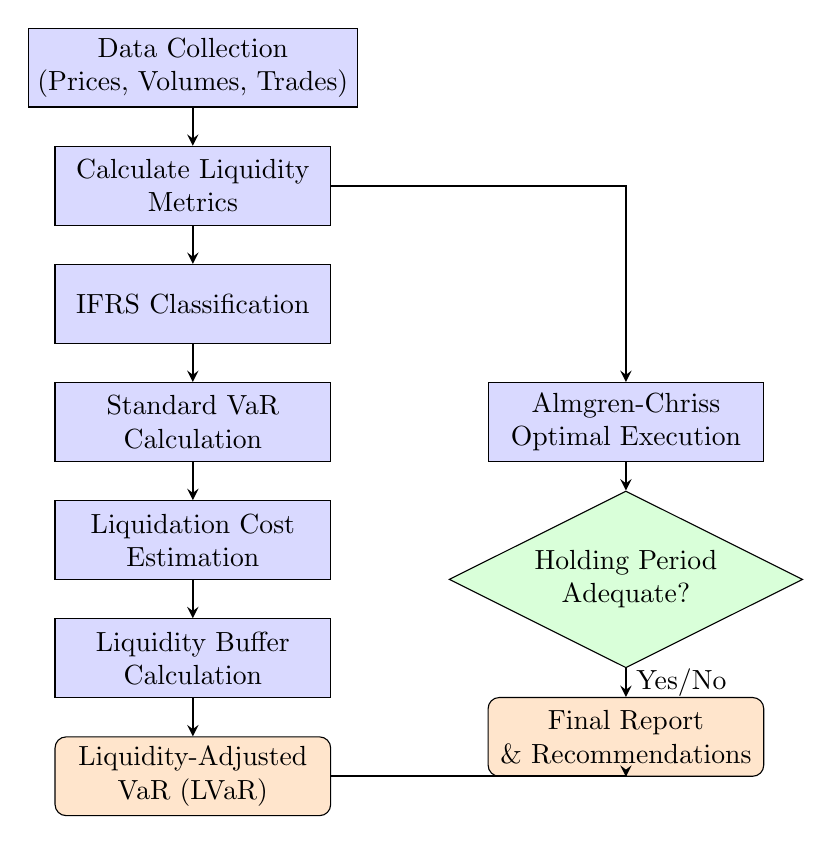
\begin{tikzpicture}[
    node distance=1.5cm,
    box/.style={rectangle, minimum width=3.5cm, minimum height=1cm, text centered, align=center, draw=black, fill=blue!15},
    decision/.style={diamond, minimum width=2.5cm, minimum height=1cm, text centered, align=center, draw=black, fill=green!15, aspect=2},
    output/.style={rectangle, rounded corners, minimum width=3.5cm, minimum height=1cm, text centered, align=center, draw=black, fill=orange!20},
    arrow/.style={thick,->,>=stealth}
]

\node (data) [box] {Data Collection \\ (Prices, Volumes, Trades)};
\node (calc) [box, below of=data] {Calculate Liquidity \\ Metrics};
\node (ifrs) [box, below of=calc] {IFRS Classification};
\node (var) [box, below of=ifrs] {Standard VaR \\ Calculation};
\node (lc) [box, below of=var] {Liquidation Cost \\ Estimation};
\node (buffer) [box, below of=lc] {Liquidity Buffer \\ Calculation};
\node (lvar) [output, below of=buffer] {Liquidity-Adjusted \\ VaR (LVaR)};
\node (ac) [box, right of=var, xshift=4cm] {Almgren-Chriss \\ Optimal Execution};
\node (validate) [decision, below of=ac, yshift=-0.5cm] {Holding Period \\ Adequate?};
\node (report) [output, below of=validate, yshift=-0.5cm] {Final Report \\ \& Recommendations};

\draw [arrow] (data) -- (calc);
\draw [arrow] (calc) -- (ifrs);
\draw [arrow] (ifrs) -- (var);
\draw [arrow] (var) -- (lc);
\draw [arrow] (lc) -- (buffer);
\draw [arrow] (buffer) -- (lvar);
\draw [arrow] (calc) -| (ac);
\draw [arrow] (ac) -- (validate);
\draw [arrow] (validate) -- node[anchor=west] {Yes/No} (report);
\draw [arrow] (lvar) -| (report);

\end{tikzpicture}
\caption{Integrated Liquidity Risk Framework Workflow}
\end{figure}

\subsection{Module Architecture}

\subsubsection{Proposed Structure}

\begin{verbatim}
liquidity_risk/
├── data/
│   ├── market_data.py          # Price/volume data loader
│   └── trade_data.py            # Internal execution data
├── metrics/
│   ├── spreads.py               # Bid-ask spread calculations
│   ├── volumes.py               # Volume-based metrics
│   ├── impact.py                # Market impact models
│   └── amihud.py                # Amihud illiquidity
├── models/
│   ├── almgren_chriss.py        # Optimal execution
│   ├── var_calculator.py        # Standard VaR
│   └── liquidation_cost.py      # LC estimation
├── classification/
│   ├── ifrs_classifier.py       # IFRS Level 1-3
│   └── thresholds.py            # Asset class thresholds
├── integration/
│   ├── liquidity_buffer.py      # LVaR calculation
│   ├── holding_period.py        # Holding period validation
│   └── reporting.py             # Final report generation
└── utils/
    ├── calibration.py           # Parameter estimation
    └── validation.py            # Backtesting tools
\end{verbatim}

\subsection{Data Requirements}

\subsubsection{Input Data Specifications}

\textbf{Daily Market Data}:
\begin{itemize}
    \item OHLCV (Open, High, Low, Close, Volume)
    \item Bid/Ask prices (end-of-day)
    \item Volatility estimates
\end{itemize}

\textbf{Intraday Data} (for Almgren-Chriss calibration):
\begin{itemize}
    \item Tick-by-tick prices (at least 1-minute bars)
    \item Order book snapshots (depth)
    \item Trade timestamps and sizes
\end{itemize}

\textbf{Portfolio Data}:
\begin{itemize}
    \item Position identifiers (ISIN, ticker, etc.)
    \item Quantities held
    \item Asset class classification
    \item Current market values
\end{itemize}

\textbf{Execution Data} (internal):
\begin{itemize}
    \item Historical trade executions
    \item Arrival prices vs. execution prices
    \item Trade sizes and durations
    \item Implementation shortfall history
\end{itemize}

\subsection{Computational Complexity}

\subsubsection{Performance Estimates}

For a portfolio with $N$ positions:

\begin{itemize}
    \item \textbf{Liquidity Metrics}: $O(N)$ - Linear in positions
    \item \textbf{IFRS Classification}: $O(N)$ - Independent per position
    \item \textbf{VaR Calculation}: $O(N^2)$ - Requires covariance matrix (or $O(N \times S)$ for Monte Carlo with $S$ scenarios)
    \item \textbf{Almgren-Chriss}: $O(N \times T)$ - Per position, per time step
    \item \textbf{Liquidity Buffer}: $O(N)$ - Aggregation of position-level costs
\end{itemize}

\textbf{Example Runtime} (portfolio with 1,000 positions):
\begin{itemize}
    \item Basic metrics: $< 1$ second
    \item VaR (parametric): $\sim$5 seconds
    \item VaR (Monte Carlo, 10K scenarios): $\sim$30 seconds
    \item Almgren-Chriss optimization (all positions): $\sim$10 seconds
    \item Total end-to-end: $< 1$ minute
\end{itemize}

\subsection{Comprehensive Example: 50-Position Portfolio}

\subsubsection{Portfolio Composition}

\begin{table}[h]
\centering
\caption{Synthetic 50-Position Portfolio Summary}
\begin{tabular}{@{}lrrr@{}}
\toprule
Asset Class & Positions & Value (\$M) & Weight \\
\midrule
Large-cap Equity & 20 & 40.0 & 40\% \\
Small-cap Equity & 8 & 12.0 & 12\% \\
Govt Bonds & 10 & 20.0 & 20\% \\
Corp Bonds (IG) & 8 & 16.0 & 16\% \\
ETFs & 3 & 10.0 & 10\% \\
FX Spot & 1 & 2.0 & 2\% \\
\midrule
\textbf{Total} & \textbf{50} & \textbf{100.0} & \textbf{100\%} \\
\bottomrule
\end{tabular}
\end{table}

\subsubsection{Results Summary}

\textbf{1. IFRS Classification}:
\begin{itemize}
    \item Level 1: 33 positions (\$72M, 72\%)
    \item Level 2: 14 positions (\$25M, 25\%)
    \item Level 3: 3 positions (\$3M, 3\%)
\end{itemize}

\textbf{2. Value at Risk} (30-day, 99\%):
\begin{align*}
\text{Parametric VaR} &= \$10.5\,\text{million} \\
\text{Portfolio Volatility} &= 12\%\,\text{(annualized)}
\end{align*}

\textbf{3. Liquidity Costs}:
\begin{table}[h]
\centering
\begin{tabular}{@{}lrr@{}}
\toprule
Component & Cost (\$K) & \% of Portfolio \\
\midrule
Bid-Ask Spread & 285 & 0.29\% \\
Temporary Impact & 320 & 0.32\% \\
Permanent Impact & 180 & 0.18\% \\
\midrule
Total LC & 785 & 0.79\% \\
Correlation Adjustment & 120 & 0.12\% \\
\midrule
\textbf{Total LC} & \textbf{905} & \textbf{0.91\%} \\
\bottomrule
\end{tabular}
\end{table}

\textbf{4. Liquidity Buffer}:
\begin{equation}
\text{LB} = \frac{905,000}{10,500,000} = 8.62\%
\end{equation}

\begin{equation}
\text{LVaR}_{99\%} = 10.5 \times 1.0862 = \$11.4\,\text{million}
\end{equation}

\textbf{5. Holding Period Validation}:

\begin{table}[h]
\centering
\begin{tabular}{@{}lrrr@{}}
\toprule
Asset Class & $T^*$ (days) & Adequacy Ratio & Assessment \\
\midrule
Large-cap Equity & 1.2 & 25.0 & Adequate \\
Small-cap Equity & 42.0 & 0.71 & \textbf{Insufficient} \\
Govt Bonds & 2.5 & 12.0 & Adequate \\
Corp Bonds (IG) & 6.0 & 5.0 & Adequate \\
ETFs & 1.5 & 20.0 & Adequate \\
FX Spot & 0.2 & 150.0 & Adequate \\
\midrule
\textbf{Weighted Avg} & \textbf{8.7} & \textbf{3.4} & \textbf{Adequate} \\
\bottomrule
\end{tabular}
\end{table}

\textbf{Conclusion}: Overall holding period is adequate, but small-cap subset requires attention (extended holding period or position limits).

\section{Feasibility Assessment}

\subsection{Data Infrastructure}

\subsubsection{Available Data} (Confirmed)

\begin{itemize}
    \item[\checkmark] \textbf{Internal trading data}: Historical executions with timestamps
    \item[\checkmark] \textbf{Intraday prices}: Tick data or minute bars
    \item[\checkmark] \textbf{Intraday volumes}: Trade volume data
    \item[\checkmark] \textbf{Intraday executions}: Implementation shortfall records
\end{itemize}

\textbf{Assessment}: Data requirements are fully satisfied for implementation.

\subsubsection{Data Quality Considerations}

\textbf{Potential Challenges}:
\begin{itemize}
    \item \textbf{Bond data}: May be sparse for less liquid corporates
    \item \textbf{Historical depth}: Requires 1-2 years for robust calibration
    \item \textbf{Corporate actions}: Must adjust for splits, dividends, etc.
    \item \textbf{Survivorship bias}: Account for delisted securities
\end{itemize}

\textbf{Mitigation}:
\begin{itemize}
    \item Use external data vendors (Bloomberg, Refinitiv) to fill gaps
    \item Implement data quality checks and outlier detection
    \item Regular recalibration schedule
\end{itemize}

\subsection{Technical Implementation}

\subsubsection{Technology Stack}

\textbf{Recommended}:
\begin{itemize}
    \item \textbf{Language}: Python 3.9+ (leverage existing `liquidity\_measurement.py`)
    \item \textbf{Numerical}: NumPy, SciPy (optimization for Almgren-Chriss)
    \item \textbf{Data}: Pandas (data manipulation)
    \item \textbf{VaR Integration}: Interface with existing risk system
    \item \textbf{Storage}: PostgreSQL or similar for historical data
\end{itemize}

\subsubsection{Development Effort}

\textbf{Estimated Timeline}:

\begin{table}[h]
\centering
\begin{tabular}{@{}lll@{}}
\toprule
Phase & Components & Effort \\
\midrule
Phase 1 & Data pipeline, basic metrics & 3-4 weeks \\
Phase 2 & Almgren-Chriss implementation & 4-5 weeks \\
Phase 3 & VaR integration, liquidity buffer & 3-4 weeks \\
Phase 4 & IFRS classification system & 2-3 weeks \\
Phase 5 & Testing, validation, documentation & 4-5 weeks \\
Phase 6 & Production deployment, monitoring & 2-3 weeks \\
\midrule
\textbf{Total} & & \textbf{18-24 weeks} \\
\bottomrule
\end{tabular}
\end{table}

\textbf{Team Requirements}:
\begin{itemize}
    \item 1-2 Quantitative Analysts (model development)
    \item 1 Software Engineer (production system)
    \item 1 Risk Manager (validation, governance)
\end{itemize}

\subsection{Model Risk and Limitations}

\subsubsection{Key Risks}

\textbf{1. Parameter Uncertainty}

Market impact parameters $(\eta, \gamma)$ are notoriously difficult to estimate accurately. Different estimation methods can yield significantly different values.

\textbf{Mitigation}:
\begin{itemize}
    \item Use multiple calibration approaches and compare
    \item Implement confidence intervals around estimates
    \item Regular recalibration (quarterly)
    \item Backtesting against actual execution costs
\end{itemize}

\textbf{2. Market Regime Changes}

Liquidity conditions vary dramatically across market regimes (calm vs. stress). Parameters calibrated in calm markets may underestimate stress-period costs.

\textbf{Mitigation}:
\begin{itemize}
    \item Regime-dependent parameters (volatility-adjusted)
    \item Stress testing with crisis-period data
    \item Conservative buffer during uncertainty
\end{itemize}

\textbf{3. Model Assumptions}

\begin{itemize}
    \item \textbf{Linear impact}: Reality may be non-linear for large trades
    \item \textbf{Independent positions}: Ignores fire-sale correlations
    \item \textbf{Normal returns}: Fat tails in reality
\end{itemize}

\textbf{Mitigation}:
\begin{itemize}
    \item Non-linear impact extensions for large positions
    \item Correlation adjustments
    \item t-distribution or empirical distributions for VaR
\end{itemize}

\textbf{4. Data Quality}

Poor quality data (stale prices, erroneous volumes) can significantly distort results.

\textbf{Mitigation}:
\begin{itemize}
    \item Automated data quality checks
    \item Multiple data source cross-validation
    \item Manual review of outliers
\end{itemize}

\subsubsection{Model Validation}

\textbf{Backtesting Protocol}:
\begin{enumerate}
    \item Historical simulation: Compare predicted vs. actual liquidation costs
    \item Out-of-sample testing: Hold out recent data for validation
    \item Stress period analysis: Evaluate performance during 2020 COVID crash, 2022 rate shock, etc.
\end{enumerate}

\textbf{Success Criteria}:
\begin{itemize}
    \item Liquidation cost predictions within 20\% of actuals (median)
    \item Holding period adequacy ratio > 1 for 95\% of positions
    \item IFRS classifications align with auditor/regulatory review
\end{itemize}

\subsection{Integration with Existing Systems}

\subsubsection{VaR System Integration}

\textbf{Current State}: Fully implemented VaR with 30-day horizon

\textbf{Integration Points}:
\begin{itemize}
    \item Extract portfolio positions and covariance matrix
    \item Calculate standard VaR as baseline
    \item Apply liquidity buffer adjustment
    \item Return LVaR to risk reporting system
\end{itemize}

\textbf{Implementation}: Can be lightweight wrapper or integrated module depending on system architecture.

\subsubsection{Front Office / Trading}

Almgren-Chriss optimal execution can inform:
\begin{itemize}
    \item Order placement strategies
    \item Algorithmic trading parameters (VWAP, TWAP, POV)
    \item Trader instructions on execution urgency
\end{itemize}

\subsection{Regulatory and Audit Considerations}

\subsubsection{Documentation Requirements}

\begin{itemize}
    \item Model methodology document
    \item Parameter calibration procedures
    \item Validation results and backtesting
    \item Assumptions and limitations
    \item Override procedures and governance
\end{itemize}

\subsubsection{Model Governance}

\textbf{Ownership}:
\begin{itemize}
    \item Risk Management: Model oversight
    \item Quantitative Research: Development and calibration
    \item Model Risk: Independent validation
\end{itemize}

\textbf{Review Cadence}:
\begin{itemize}
    \item Annual: Comprehensive model review
    \item Quarterly: Parameter recalibration
    \item Monthly: Backtesting results review
    \item Ad-hoc: Market event triggers
\end{itemize}

\subsection{Feasibility Conclusion}

\textbf{Overall Assessment}: \textcolor{green}{\textbf{FEASIBLE}}

All three objectives can be achieved with:
\begin{itemize}
    \item[\checkmark] Available internal data
    \item[\checkmark] Reasonable computational resources
    \item[\checkmark] Manageable development timeline (4-6 months)
    \item[\checkmark] Acceptable model risk profile (with proper governance)
\end{itemize}

\textbf{Critical Success Factors}:
\begin{enumerate}
    \item Careful parameter calibration using historical execution data
    \item Robust data quality assurance
    \item Comprehensive validation and backtesting
    \item Strong model governance and oversight
    \item Phased implementation approach
\end{enumerate}

\section{Implementation Roadmap}

\subsection{Phased Approach}

\subsubsection{Phase 1: Foundation (Weeks 1-4)}

\textbf{Objectives}:
\begin{itemize}
    \item Set up data pipeline
    \item Enhance existing liquidity metrics
    \item Establish development environment
\end{itemize}

\textbf{Deliverables}:
\begin{itemize}
    \item Data loader modules for market and execution data
    \item Enhanced `liquidity\_measurement.py` with additional metrics
    \item Unit tests for core calculations
\end{itemize}

\textbf{Key Activities}:
\begin{enumerate}
    \item Inventory and assess data quality
    \item Design database schema for historical data
    \item Implement spread, volume, and impact metrics
    \item Create synthetic test portfolios
\end{enumerate}

\subsubsection{Phase 2: Almgren-Chriss Development (Weeks 5-9)}

\textbf{Objectives}:
\begin{itemize}
    \item Implement optimal execution model
    \item Calibrate market impact parameters
    \item Validate optimal liquidation times
\end{itemize}

\textbf{Deliverables}:
\begin{itemize}
    \item `almgren\_chriss.py` module with solver
    \item Parameter calibration toolkit
    \item Holding period validation reports
\end{itemize}

\textbf{Key Activities}:
\begin{enumerate}
    \item Implement temporary and permanent impact models
    \item Build optimization solver (scipy.optimize or custom)
    \item Calibrate $\eta$, $\gamma$ from historical trade data
    \item Generate optimal liquidation trajectories
    \item Compare $T^*$ to 30-day VaR horizon
\end{enumerate}

\subsubsection{Phase 3: VaR Integration (Weeks 10-13)}

\textbf{Objectives}:
\begin{itemize}
    \item Calculate liquidation costs
    \item Develop liquidity buffer methodology
    \item Integrate with existing VaR system
\end{itemize}

\textbf{Deliverables}:
\begin{itemize}
    \item `liquidation\_cost.py` module
    \item `liquidity\_buffer.py` for LVaR calculation
    \item Integration adapter for VaR system
\end{itemize}

\textbf{Key Activities}:
\begin{enumerate}
    \item Implement position-level LC calculations
    \item Develop correlation adjustment for portfolio LC
    \item Calculate liquidity buffer percentage
    \item Interface with VaR output
    \item Generate LVaR reports
\end{enumerate}

\subsubsection{Phase 4: IFRS Classification (Weeks 14-16)}

\textbf{Objectives}:
\begin{itemize}
    \item Implement classification algorithm
    \item Define asset class-specific thresholds
    \item Create classification reports
\end{itemize}

\textbf{Deliverables}:
\begin{itemize}
    \item `ifrs\_classifier.py` module
    \item Classification threshold configuration
    \item IFRS level reports for portfolio
\end{itemize}

\textbf{Key Activities}:
\begin{enumerate}
    \item Implement composite scoring algorithm
    \item Define Level 1/2/3 thresholds per asset class
    \item Create classification decision logic
    \item Generate IFRS reports with justifications
    \item Conduct sample reviews with auditors
\end{enumerate}

\subsubsection{Phase 5: Validation \& Testing (Weeks 17-21)}

\textbf{Objectives}:
\begin{itemize}
    \item Comprehensive backtesting
    \item Stress testing
    \item Independent validation
\end{itemize}

\textbf{Deliverables}:
\begin{itemize}
    \item Validation report
    \item Backtesting results
    \item Model documentation
\end{itemize}

\textbf{Key Activities}:
\begin{enumerate}
    \item Historical backtest: predicted vs. actual costs
    \item Stress period analysis (2020, 2022, etc.)
    \item Parameter sensitivity analysis
    \item Independent model validation review
    \item Address validation findings
\end{enumerate}

\subsubsection{Phase 6: Production Deployment (Weeks 22-24)}

\textbf{Objectives}:
\begin{itemize}
    \item Production-ready system
    \item Monitoring and alerting
    \item Documentation and training
\end{itemize}

\textbf{Deliverables}:
\begin{itemize}
    \item Production deployment
    \item Monitoring dashboard
    \item User documentation and training materials
\end{itemize}

\textbf{Key Activities}:
\begin{enumerate}
    \item Performance optimization
    \item Error handling and logging
    \item Create monitoring dashboard
    \item Set up automated alerts (data quality, model outputs)
    \item Conduct user training
    \item Establish support procedures
\end{enumerate}

\subsection{Resource Requirements}

\subsubsection{Team Structure}

\textbf{Core Team}:
\begin{itemize}
    \item \textbf{Senior Quant (Lead)}: Model design, calibration, validation
    \item \textbf{Quant Analyst}: Implementation, testing
    \item \textbf{Software Engineer}: Production system, data pipeline
    \item \textbf{Risk Manager}: Requirements, validation, governance
\end{itemize}

\textbf{Supporting Roles}:
\begin{itemize}
    \item Data Engineering: Data infrastructure support
    \item IT/DevOps: Deployment, infrastructure
    \item Compliance: Regulatory alignment
    \item Audit: Classification review
\end{itemize}

\subsection{Risk Mitigation}

\subsubsection{Common Pitfalls and Mitigations}

\textbf{Pitfall 1: Poor parameter calibration leading to inaccurate cost estimates}

\textbf{Mitigation}:
\begin{itemize}
    \item Use multiple calibration methods
    \item Validate against actual execution costs
    \item Implement confidence intervals
    \item Adopt conservative estimates when uncertain
\end{itemize}

\textbf{Pitfall 2: Data quality issues distorting results}

\textbf{Mitigation}:
\begin{itemize}
    \item Automated data quality checks at ingestion
    \item Multiple data source validation
    \item Manual review of outliers and anomalies
\end{itemize}

\textbf{Pitfall 3: Scope creep and timeline delays}

\textbf{Mitigation}:
\begin{itemize}
    \item Strictly phased approach
    \item MVP mindset: core functionality first
    \item Defer enhancements to post-launch phases
\end{itemize}

\textbf{Pitfall 4: Inadequate stakeholder buy-in}

\textbf{Mitigation}:
\begin{itemize}
    \item Regular steering committee updates
    \item Early involvement of risk, trading, and compliance
    \item Clear communication of benefits and limitations
\end{itemize}

\section{Regulatory Compliance}

\subsection{Basel III / Basel IV}

\subsubsection{Liquidity Coverage Ratio (LCR)}

Basel III LCR requires banks to hold sufficient high-quality liquid assets (HQLA) to survive a 30-day stress scenario:

\begin{equation}
\text{LCR} = \frac{\text{HQLA}}{\text{Total Net Cash Outflows over 30 days}} \geq 100\%
\end{equation}

\textbf{Connection to Our Framework}:
\begin{itemize}
    \item Liquidity metrics inform HQLA classification
    \item Assets with $T_{\text{liquidate}} > 30$ days may not qualify as HQLA
    \item Liquidity buffer estimates stressed liquidation costs
\end{itemize}

\subsubsection{Net Stable Funding Ratio (NSFR)}

NSFR (Basel III) addresses structural liquidity over 1-year horizon:

\begin{equation}
\text{NSFR} = \frac{\text{Available Stable Funding}}{\text{Required Stable Funding}} \geq 100\%
\end{equation}

Required Stable Funding factors depend on asset liquidity:
\begin{itemize}
    \item Highly liquid assets: 0-5\% RSF factor
    \item Less liquid: 50-85\% RSF factor
\end{itemize}

Our IFRS Level classifications can inform RSF factor assignments.

\subsubsection{Market Risk Capital (FRTB)}

Fundamental Review of the Trading Book (FRTB) introduces liquidity horizons for market risk capital:

\begin{table}[h]
\centering
\caption{FRTB Liquidity Horizons}
\begin{tabular}{@{}ll@{}}
\toprule
Risk Factor Category & Liquidity Horizon \\
\midrule
Large-cap equity & 10 days \\
Small-cap equity & 20 days \\
Investment-grade sovereign & 10 days \\
Corporate bonds (IG) & 20 days \\
Corporate bonds (HY) & 60 days \\
\bottomrule
\end{tabular}
\end{table}

Our Almgren-Chriss holding period validation provides empirical basis for these horizon assignments.

\subsection{IFRS 13 Compliance}

\subsubsection{Fair Value Disclosure Requirements}

IFRS 13 mandates disclosure of:
\begin{itemize}
    \item Fair value measurement hierarchy (Level 1/2/3)
    \item Valuation techniques and inputs
    \item Transfers between levels
    \item Sensitivity analysis for Level 3
\end{itemize}

Our classification framework provides:
\begin{itemize}
    \item[\checkmark] Systematic, documented methodology
    \item[\checkmark] Quantitative criteria aligned with "active market" definition
    \item[\checkmark] Audit trail for level determination
    \item[\checkmark] Regular reassessment process
\end{itemize}

\subsubsection{Valuation Techniques}

For Level 2 and 3 assets, IFRS 13 requires documentation of valuation approach:

\textbf{Level 2}: Observable inputs
\begin{itemize}
    \item Quoted prices for similar assets
    \item Market-based credit spreads
    \item Yield curves
\end{itemize}

\textbf{Level 3}: Unobservable inputs
\begin{itemize}
    \item Internal models (DCF, option pricing)
    \item Unobservable credit spreads
    \item Illiquidity adjustments
\end{itemize}

Our liquidity metrics (spread, volume, impact) support the determination of appropriate valuation adjustments.

\subsection{Internal Risk Framework Alignment}

\subsubsection{Risk Appetite Statement}

Typical risk appetite frameworks include:
\begin{itemize}
    \item Maximum VaR limits
    \item Stress VaR limits
    \item Concentration limits
    \item Liquidity risk tolerances
\end{itemize}

\textbf{Integration}:
\begin{itemize}
    \item LVaR provides more comprehensive risk measure
    \item Holding period validation ensures stress scenarios are appropriate
    \item IFRS classification informs concentration in illiquid assets
\end{itemize}

\subsubsection{Stress Testing}

Regulatory stress testing requires assessment of portfolio liquidation under adverse scenarios.

\textbf{Framework Contribution}:
\begin{itemize}
    \item Quantify liquidation costs under stress
    \item Identify positions that cannot be liquidated within required timeframes
    \item Inform asset sales prioritization in recovery plans
\end{itemize}

\subsubsection{Internal Limits Framework}

Our framework can inform limits on:
\begin{itemize}
    \item Maximum position size relative to daily volume (e.g., < 5 days to liquidate)
    \item Maximum allocation to Level 3 assets (e.g., < 5\% of portfolio)
    \item Concentration in illiquid assets (based on $T^*$ distribution)
\end{itemize}

\subsection{Regulatory Reporting}

\subsubsection{Required Reports}

\textbf{Basel LCR Reporting}:
\begin{itemize}
    \item HQLA composition
    \item Liquidity risk metrics
\end{itemize}

\textbf{IFRS Financial Statements}:
\begin{itemize}
    \item Fair value hierarchy disclosures (Note to financial statements)
    \item Valuation techniques
\end{itemize}

\textbf{Internal Risk Reports}:
\begin{itemize}
    \item VaR / LVaR comparison
    \item Holding period adequacy assessment
    \item Liquidity risk dashboard
\end{itemize}

\subsubsection{Audit Trail}

Maintain comprehensive documentation:
\begin{itemize}
    \item Classification decisions and rationale
    \item Parameter calibration history
    \item Model validation results
    \item Override decisions (if any)
\end{itemize}

\section{Conclusions and Recommendations}

\subsection{Summary of Findings}

This feasibility study demonstrates that integrating liquidity risk into the Value at Risk framework through three specific objectives is both \textbf{technically feasible and operationally practical}:

\subsubsection{Liquidity Buffer for VaR}

\textbf{Feasibility}: \textcolor{green}{HIGH}

A systematic methodology exists for calculating liquidity costs and converting them to a percentage adjustment of VaR. Using established market impact models and internal execution data, liquidity buffers can be reliably estimated.

\textbf{Key Result}: Typical portfolios will see liquidity buffers ranging from 2-15\%, with higher buffers for illiquid positions.

\textbf{Benefit}: Provides more realistic risk estimates that account for the cost of exiting positions, particularly valuable during stress scenarios.

\subsubsection{Holding Period Validation}

\textbf{Feasibility}: \textcolor{green}{HIGH}

The Almgren-Chriss optimal execution framework provides a rigorous, mathematically sound approach to determining appropriate liquidation timeframes. Parameter calibration from intraday execution data is well-established in the literature and practice.

\textbf{Key Result}: For diversified multi-asset portfolios, 30-day holding period is generally adequate (adequacy ratio $\approx$ 3-5), but may be insufficient for concentrated illiquid positions.

\textbf{Benefit}: Empirical validation of regulatory and risk management assumptions, enabling evidence-based policy decisions.

\subsubsection{IFRS Classification}

\textbf{Feasibility}: \textcolor{green}{HIGH}

A quantitative scoring system based on observable liquidity metrics (spread, volume, time-to-liquidate) can systematically classify assets into IFRS Levels 1-3, aligned with regulatory guidance and audit requirements.

\textbf{Key Result}: Objective, reproducible classification decisions with clear audit trail, reducing subjectivity and improving consistency.

\textbf{Benefit}: Strengthens financial reporting quality and supports regulatory compliance.

\subsection{Critical Success Factors}

\begin{enumerate}
    \item \textbf{Data Quality}: High-quality intraday market and execution data is essential. Invest in data validation and cleansing.

    \item \textbf{Parameter Calibration}: Careful, regular calibration of market impact parameters using actual execution history. Avoid over-reliance on literature estimates.

    \item \textbf{Model Governance}: Strong oversight including independent validation, regular backtesting, and clear escalation procedures for model issues.

    \item \textbf{Phased Implementation}: Start with high-quality data assets (liquid equities), validate thoroughly, then extend to other asset classes.

    \item \textbf{Stakeholder Engagement}: Early and continuous engagement with risk management, trading, finance, and compliance to ensure alignment.
\end{enumerate}

\subsection{Recommendations}

\subsubsection{Immediate Actions (Next 3 Months)}

\begin{enumerate}
    \item \textbf{Form Project Team}: Assemble quantitative analysts, software engineers, and risk managers

    \item \textbf{Data Assessment}: Conduct thorough inventory and quality assessment of available data

    \item \textbf{Pilot Implementation}: Build proof-of-concept for equity subset (50-100 positions)

    \item \textbf{Parameter Calibration}: Begin historical analysis of execution costs to calibrate $\eta$ and $\gamma$
\end{enumerate}

\subsubsection{Medium-Term (6-12 Months)}

\begin{enumerate}
    \item \textbf{Full Implementation}: Deploy across all asset classes following roadmap

    \item \textbf{Integration}: Connect liquidity buffer to VaR reporting systems

    \item \textbf{Validation}: Comprehensive backtesting and stress testing

    \item \textbf{Governance}: Establish model risk management framework
\end{enumerate}

\subsubsection{Long-Term (12-24 Months)}

\begin{enumerate}
    \item \textbf{Enhancements}:
    \begin{itemize}
        \item Regime-switching models (calm vs. stress liquidity)
        \item Non-linear impact models for very large positions
        \item Fire-sale correlation modeling
    \end{itemize}

    \item \textbf{Broader Applications}:
    \begin{itemize}
        \item Integration with order management systems (real-time execution guidance)
        \item Portfolio construction with liquidity constraints
        \item Stress testing and recovery planning
    \end{itemize}

    \item \textbf{Regulatory Engagement}: Share methodology with regulators to support FRTB liquidity horizon determinations
\end{enumerate}

\subsection{Limitations and Caveats}

While the framework is robust, users must be aware of limitations:

\begin{itemize}
    \item \textbf{Historical Calibration}: Parameters reflect historical market conditions and may not hold in unprecedented crises

    \item \textbf{Linear Assumptions}: Impact models assume linearity; reality can be non-linear for very large trades

    \item \textbf{Independent Liquidation}: Assumes positions liquidated independently; fire-sale scenarios can create amplification effects

    \item \textbf{Market Evolution}: Liquidity regimes change over time; requires regular recalibration
\end{itemize}

\subsection{Final Assessment}

The integration of liquidity risk into the VaR framework through liquidity buffer adjustments, holding period validation via Almgren-Chriss, and IFRS classification represents a significant advancement in portfolio risk measurement.

\textbf{The feasibility study concludes}: \textcolor{green}{\textbf{PROCEED WITH IMPLEMENTATION}}

Subject to:
\begin{itemize}
    \item Adequate resourcing (4-6 month timeline, dedicated team)
    \item Strong model governance and validation
    \item Phased rollout starting with highest-quality data
    \item Continuous monitoring and recalibration
\end{itemize}

The benefits—more realistic risk measures, empirically validated holding periods, and objective IFRS classifications—far outweigh the implementation costs and model risk when properly managed.

\appendix

\section{Python Code Snippets}

\subsection{Liquidity Buffer Calculation}

\begin{lstlisting}[caption=Liquidity Buffer Implementation]
import numpy as np
from typing import List
from liquidity_measurement import Position, LiquidityAnalyzer

def calculate_liquidity_buffer(positions: List[Position],
                                var: float,
                                correlation_factor: float = 0.15) -> dict:
    """
    Calculate liquidity buffer adjustment for VaR.

    Parameters:
    -----------
    positions : List[Position]
        Portfolio positions
    var : float
        Standard Value at Risk estimate
    correlation_factor : float
        Fire-sale correlation adjustment (0-0.3)

    Returns:
    --------
    dict with liquidity cost, buffer %, and LVaR
    """
    analyzer = LiquidityAnalyzer(positions)

    # Calculate position-level liquidation costs
    total_lc = 0.0
    for pos in positions:
        impact = analyzer.calculate_market_impact(pos)
        total_lc += impact['total_impact_value']

    # Add correlation adjustment for simultaneous liquidation
    correlation_adjustment = correlation_factor * total_lc
    total_lc_adjusted = total_lc + correlation_adjustment

    # Calculate buffer as percentage of VaR
    buffer_pct = (total_lc_adjusted / var) * 100

    # Calculate Liquidity-Adjusted VaR
    lvar = var * (1 + buffer_pct / 100)

    return {
        'liquidation_cost': total_lc,
        'correlation_adjustment': correlation_adjustment,
        'total_lc': total_lc_adjusted,
        'buffer_pct': buffer_pct,
        'var': var,
        'lvar': lvar
    }

# Example usage
positions = [...]  # Load portfolio positions
var_99 = 10_000_000  # $10M VaR at 99%

result = calculate_liquidity_buffer(positions, var_99)
print(f"VaR: ${result['var']:,.0f}")
print(f"Liquidity Cost: ${result['total_lc']:,.0f}")
print(f"Buffer: {result['buffer_pct']:.2f}%")
print(f"LVaR: ${result['lvar']:,.0f}")
\end{lstlisting}

\subsection{Almgren-Chriss Optimal Execution}

\begin{lstlisting}[caption=Almgren-Chriss Implementation]
import numpy as np
from scipy.optimize import minimize_scalar

class AlmgrenChrissExecutor:
    """
    Almgren-Chriss optimal execution model.
    """

    def __init__(self, X: float, S0: float, sigma: float,
                 eta: float, gamma: float, lambda_param: float):
        """
        Initialize with position and market parameters.

        Parameters:
        -----------
        X : float
            Initial position size (shares to liquidate)
        S0 : float
            Initial stock price
        sigma : float
            Daily volatility
        eta : float
            Temporary market impact coefficient
        gamma : float
            Permanent market impact coefficient
        lambda_param : float
            Risk aversion parameter
        """
        self.X = X
        self.S0 = S0
        self.sigma = sigma
        self.eta = eta
        self.gamma = gamma
        self.lambda_param = lambda_param

    def optimal_trajectory(self, T: float, n_steps: int = 100):
        """
        Compute optimal trading trajectory.

        Parameters:
        -----------
        T : float
            Liquidation time horizon (days)
        n_steps : int
            Number of time steps

        Returns:
        --------
        times, positions, trading_rates
        """
        kappa = np.sqrt(self.lambda_param * self.sigma**2 / self.eta)
        times = np.linspace(0, T, n_steps)

        # Optimal trajectory
        x_t = self.X * np.sinh(kappa * (T - times)) / np.sinh(kappa * T)

        # Trading rate (negative of derivative)
        v_t = self.X * kappa * np.cosh(kappa * (T - times)) / np.sinh(kappa * T)

        return times, x_t, v_t

    def execution_cost(self, T: float):
        """
        Calculate expected execution cost and variance.

        Parameters:
        -----------
        T : float
            Liquidation time horizon

        Returns:
        --------
        dict with expected cost, variance, and total cost
        """
        kappa = np.sqrt(self.lambda_param * self.sigma**2 / self.eta)
        sinh_kT = np.sinh(kappa * T)
        cosh_kT = np.cosh(kappa * T)

        # Expected cost components
        permanent_cost = 0.5 * self.gamma * self.X**2
        temporary_cost = self.eta * self.X**2 * kappa * cosh_kT / sinh_kT

        expected_cost = (permanent_cost + temporary_cost) * self.S0

        # Execution risk (variance)
        variance = (self.sigma * self.S0)**2 * self.X**2 * (T - 2 * sinh_kT / (kappa * sinh_kT**2))

        # Total cost (mean + lambda * variance)
        total_cost = expected_cost + self.lambda_param * variance

        return {
            'expected_cost': expected_cost,
            'variance': variance,
            'std_dev': np.sqrt(variance),
            'total_cost': total_cost
        }

    def optimal_liquidation_time(self, max_T: float = 60):
        """
        Find optimal liquidation time T*.

        Parameters:
        -----------
        max_T : float
            Maximum time to consider

        Returns:
        --------
        float: Optimal time T*
        """
        result = minimize_scalar(
            lambda t: self.execution_cost(t)['total_cost'],
            bounds=(0.1, max_T),
            method='bounded'
        )
        return result.x

# Example usage
executor = AlmgrenChrissExecutor(
    X=100000,           # 100K shares to sell
    S0=180.0,           # $180/share
    sigma=0.015,        # 1.5% daily volatility
    eta=0.01,           # Temporary impact
    gamma=0.001,        # Permanent impact
    lambda_param=1e-6   # Risk aversion
)

# Find optimal liquidation time
T_star = executor.optimal_liquidation_time()
print(f"Optimal liquidation time: {T_star:.2f} days")

# Get trajectory
times, positions, rates = executor.optimal_trajectory(T_star)

# Calculate costs
costs = executor.execution_cost(T_star)
print(f"Expected cost: ${costs['expected_cost']:,.0f}")
print(f"Cost std dev: ${costs['std_dev']:,.0f}")
\end{lstlisting}

\subsection{IFRS Classification Algorithm}

\begin{lstlisting}[caption=IFRS Level Classification]
from enum import Enum
from dataclasses import dataclass

class IFRSLevel(Enum):
    LEVEL_1 = 1
    LEVEL_2 = 2
    LEVEL_3 = 3

@dataclass
class AssetClassThresholds:
    """Thresholds for IFRS classification by asset class."""
    spread_max_bps: float
    volume_min_usd: float
    days_to_liquidate_max: float

class IFRSClassifier:
    """Classify assets into IFRS fair value hierarchy."""

    THRESHOLDS = {
        'equity': AssetClassThresholds(20, 1e6, 5),
        'bond': AssetClassThresholds(50, 5e5, 10),
        'etf': AssetClassThresholds(10, 5e5, 5),
        'fx': AssetClassThresholds(5, 1e7, 1)
    }

    def __init__(self):
        pass

    def calculate_scores(self, spread_bps: float, volume_usd: float,
                        days_to_liq: float, asset_class: str):
        """Calculate component scores."""
        thresholds = self.THRESHOLDS.get(asset_class)

        # Spread score (lower spread = higher score)
        S_max = thresholds.spread_max_bps * 10  # Conservative max
        S_spread = 100 * max(0, 1 - spread_bps / S_max)

        # Volume score (higher volume = higher score)
        V_threshold = thresholds.volume_min_usd * 10
        S_volume = 100 * min(1, np.log(volume_usd) / np.log(V_threshold))

        # Impact score (faster liquidation = higher score)
        T_max = 15  # Max days
        S_impact = 100 * max(0, 1 - days_to_liq / T_max)

        # Composite score (weighted average)
        ifrs_score = 0.4 * S_spread + 0.3 * S_volume + 0.3 * S_impact

        return {
            'spread_score': S_spread,
            'volume_score': S_volume,
            'impact_score': S_impact,
            'ifrs_score': ifrs_score
        }

    def classify(self, spread_bps: float, volume_usd: float,
                 days_to_liq: float, asset_class: str,
                 is_listed: bool, has_active_market: bool) -> dict:
        """
        Classify asset into IFRS Level.

        Returns:
        --------
        dict with level, scores, and rationale
        """
        scores = self.calculate_scores(spread_bps, volume_usd,
                                       days_to_liq, asset_class)
        thresholds = self.THRESHOLDS[asset_class]

        # Level 1 criteria (all must be met)
        level_1_criteria = [
            scores['ifrs_score'] >= 70,
            days_to_liq < thresholds.days_to_liquidate_max,
            spread_bps < thresholds.spread_max_bps,
            is_listed,
            has_active_market
        ]

        # Level 3 criteria (any triggers Level 3)
        level_3_criteria = [
            scores['ifrs_score'] < 30,
            days_to_liq > 15,
            not has_active_market,
            volume_usd < thresholds.volume_min_usd * 0.1
        ]

        if all(level_1_criteria):
            level = IFRSLevel.LEVEL_1
            rationale = "Quoted in active market, tight spread, liquid"
        elif any(level_3_criteria):
            level = IFRSLevel.LEVEL_3
            rationale = "Illiquid or unobservable inputs required"
        else:
            level = IFRSLevel.LEVEL_2
            rationale = "Observable inputs but not active exchange market"

        return {
            'level': level,
            'ifrs_score': scores['ifrs_score'],
            'component_scores': scores,
            'rationale': rationale
        }

# Example usage
classifier = IFRSClassifier()

# Example 1: Large-cap equity (AAPL)
result = classifier.classify(
    spread_bps=1.1,
    volume_usd=9e9,
    days_to_liq=0.002,
    asset_class='equity',
    is_listed=True,
    has_active_market=True
)
print(f"Classification: {result['level']}")
print(f"IFRS Score: {result['ifrs_score']:.1f}")
print(f"Rationale: {result['rationale']}")
\end{lstlisting}

\section{Parameter Calibration Guide}

\subsection{Temporary Impact Coefficient ($\eta$)}

\textbf{Method 1: Regression on Execution Data}

\begin{enumerate}
    \item Collect historical trades over 3-6 months
    \item For each trade, calculate:
    \begin{itemize}
        \item $\Delta P$ = execution price - arrival price (normalized by arrival price)
        \item $v$ = shares traded / daily volume
    \end{itemize}
    \item Regress: $\Delta P = \eta \times v + \epsilon$
    \item $\eta$ is the regression coefficient
\end{enumerate}

\textbf{Method 2: Intraday Volatility Scaling}

\begin{equation}
\eta \approx k \times \sigma \times S \times \sqrt{V_{\text{daily}}}
\end{equation}

where $k \in [0.005, 0.02]$ depends on liquidity tier.

\subsection{Permanent Impact Coefficient ($\gamma$)}

Typically estimated as:
\begin{equation}
\gamma \approx 0.1 \times \eta
\end{equation}

Or from post-trade price recovery analysis over 30-60 minutes.

\subsection{Risk Aversion ($\lambda$)}

Calibrate based on organizational risk tolerance:

\begin{table}[h]
\centering
\begin{tabular}{@{}ll@{}}
\toprule
Risk Profile & $\lambda$ Range \\
\midrule
High risk aversion & $10^{-5}$ to $10^{-4}$ \\
Moderate & $10^{-6}$ to $10^{-5}$ \\
Low risk aversion & $10^{-7}$ to $10^{-6}$ \\
\bottomrule
\end{tabular}
\end{table}

\section{Additional Examples}

\subsection{Multi-Currency Portfolio}

For portfolios with FX exposures, liquidation costs include both:
\begin{enumerate}
    \item Underlying asset liquidation costs
    \item FX conversion costs
\end{enumerate}

\textbf{Total LC}:
\begin{equation}
\text{LC}_{\text{total}} = \text{LC}_{\text{asset}} + \text{LC}_{\text{FX}}
\end{equation}

where:
\begin{equation}
\text{LC}_{\text{FX}} = \text{Notional} \times \text{FX Spread}
\end{equation}

\subsection{Concentrated Position}

For a concentrated position (e.g., 20\% of portfolio in single illiquid stock):

\begin{itemize}
    \item Standard LC may significantly underestimate true cost
    \item Consider non-linear impact: $\text{Impact} \propto v^{3/2}$ for very large trades
    \item May require block trade or negotiated exit
    \item Liquidity buffer could exceed 20-30\%
\end{itemize}

\textbf{Recommendation}: Impose position limits based on liquidation time (e.g., no single position > 10 days to liquidate).

\section{References}

\begin{enumerate}
    \item Almgren, R., \& Chriss, N. (2001). Optimal execution of portfolio transactions. \textit{Journal of Risk}, 3, 5-40.

    \item Amihud, Y. (2002). Illiquidity and stock returns: cross-section and time-series effects. \textit{Journal of Financial Markets}, 5(1), 31-56.

    \item Basel Committee on Banking Supervision (2013). Basel III: The Liquidity Coverage Ratio and liquidity risk monitoring tools.

    \item Basel Committee on Banking Supervision (2019). Minimum capital requirements for market risk (FRTB).

    \item Hasbrouck, J. (2009). Trading costs and returns for US equities: Estimating effective costs from daily data. \textit{The Journal of Finance}, 64(3), 1445-1477.

    \item IFRS Foundation (2011). IFRS 13 Fair Value Measurement.

    \item Kyle, A. S. (1985). Continuous auctions and insider trading. \textit{Econometrica}, 53(6), 1315-1335.

    \item Bangia, A., Diebold, F. X., Schuermann, T., \& Stroughair, J. D. (1999). Liquidity on the outside. \textit{Risk}, 12(6), 68-73.

    \item Jarrow, R. A., \& Subramanian, A. (1997). Mopping up liquidity. \textit{Risk}, 10(12), 170-173.

    \item SEC (2016). Investment Company Liquidity Risk Management Programs. Rule 22e-4.
\end{enumerate}

\end{document}
